% Questo file contiene la domanda e risposta sul Modello ER, Normalizzazione e SQL per Commissione/Candidati.
% Sarà incluso da domande_ed_esercizi_bd.tex.

\subsection*{Domanda: Modello ER, Normalizzazione e SQL (Commissione d'Esame di Stato)}

\textbf{Domanda}: Il candidato descriva il modello concettuale Entità-Relazione (ER) e il concetto di forma normale nella progettazione logica. Produca un diagramma ER per una base di dati che tenga conto per ogni sessione dell’esame di stato, i membri effettivi della commissione e i candidati, e per ogni esame memorizzi la data e i nomi dei candidati che lo hanno superato. Successivamente il candidato fornisca una progettazione in forma tabellare del modello, normalizzando le relazioni, fornendo infine una query SQL per ottenere l’elenco di tutti gli candidati che hanno superato l’esame.

\paragraph{Risposta}:

\textbf{Descrizione del Modello Concettuale Entità-Relazione (ER)}
Il \textbf{Modello Entità-Relazione (ER)} è uno strumento di alto livello per la progettazione concettuale di database. Permette di rappresentare il mondo reale tramite entità (oggetti o concetti di interesse) e relazioni (associazioni tra entità). I suoi componenti principali sono:
\begin{itemize}
    \item \textbf{Entità}: Rappresentano "cose" o "oggetti" reali (es. Candidato, Esame di stato, Membro Commissione). Rappresentate con rettangoli.
    \item \textbf{Attributi}: Proprietà delle entità o relazioni (es. Nome, Cognome, Data, Esito). Rappresentati con ovali.
    \item \textbf{Relazioni}: Associazioni logiche tra entità (es. Sostiene, Scrutina). Rappresentate con rombi. Hanno cardinalità (min:max) e partecipazione.
\end{itemize}

\paragraph{Concetto di Forma Normale nella Progettazione Logica}
La \textbf{normalizzazione} è un processo di organizzazione dei dati in un database relazionale per ridurre la ridondanza e migliorare l'integrità dei dati. Si basa sulle forme normali:
\begin{itemize}
    \item \textbf{Prima Forma Normale (1NF)}: Tutti gli attributi sono atomici e ogni record è unico.
    \item \textbf{Seconda Forma Normale (2NF)}: È in 1NF e tutti gli attributi non-chiave dipendono completamente dalla chiave primaria (no dipendenze parziali).
    \item \textbf{Terza Forma Normale (3NF)}: È in 2NF e non contiene dipendenze transitive (nessun attributo non-chiave dipende da un altro attributo non-chiave).
\end{itemize}

\paragraph{Diagramma ER per il Contesto Specifico}
Il contesto da modellare è la gestione delle sessioni d'esame di stato, dei membri della commissione, dei candidati, e il tracciamento dei candidati che hanno superato l'esame.

\begin{figure}[h!]
    \centering
    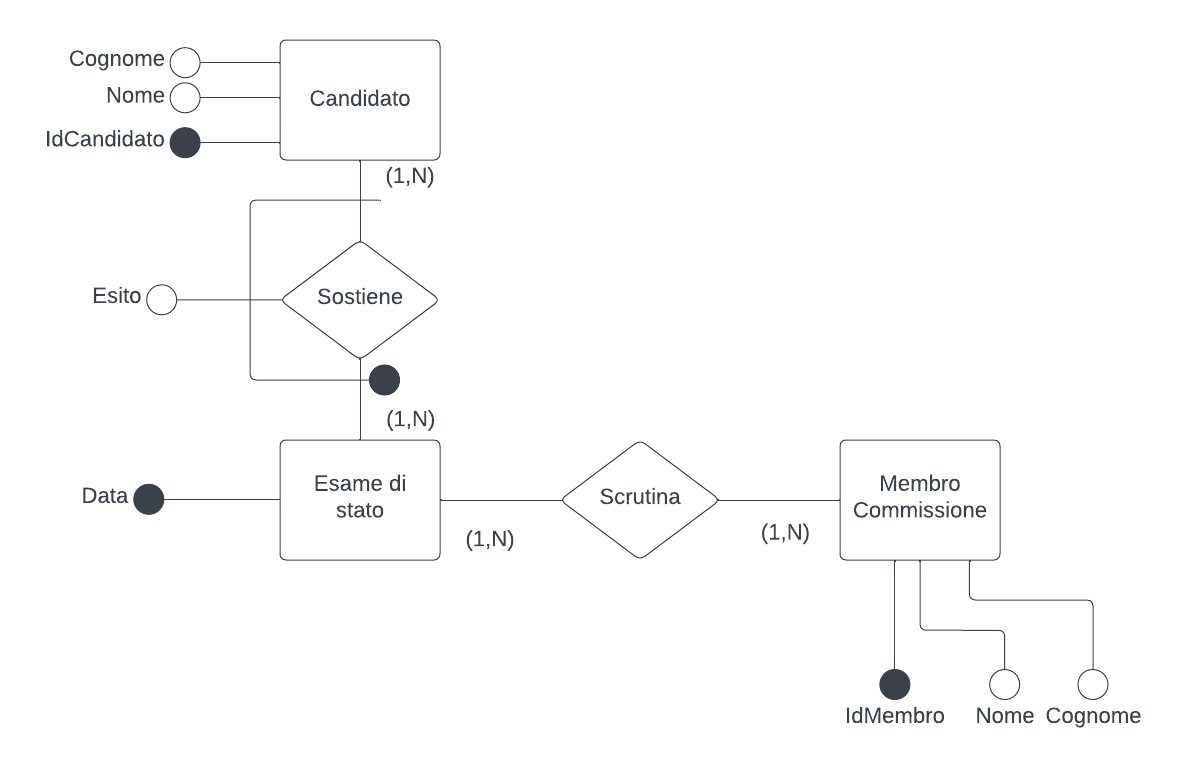
\includegraphics[width=0.9\textwidth]{capitoli/basi_di_dati/domande_teoriche/immagini/er_esame_stato_commissione_candidati.png}
    \caption{Diagramma Entità-Relazione per la gestione delle sessioni dell'Esame di Stato, Commissione e Candidati.}
    \label{fig:er_esame_stato_commissione_candidati}
\end{figure}

\textbf{Spiegazione del Diagramma:}
\begin{itemize}
    \item \textbf{Entità `Candidato`}: Rappresenta i partecipanti all'esame. Attributi: \lstinline{IdCandidato} (PK), \lstinline{Nome}, \lstinline{Cognome}.
    \item \textbf{Entità `Esame di stato`}: Rappresenta le singole sessioni d'esame. Attributi: \lstinline{Data} (PK).
    \item \textbf{Entità `Membro Commissione`}: Rappresenta i membri che compongono la commissione d'esame. Attributi: \lstinline{IdMembro} (PK), \lstinline{Nome}, \lstinline{Cognome}.
    \item \textbf{Relazione "Sostiene" (Candidato - Esame di stato)}: Relazione N:M.
    \begin{itemize}
        \item Cardinalità: Un \lstinline{Candidato} può sostenere uno o più \lstinline{Esami di stato} (\lstinline{(1,N)} lato Candidato). Un \lstinline{Esame di stato} è sostenuto da uno o più \lstinline{Candidati} (\lstinline{(1,N)} lato Esame di stato).
        \item Attributo: \lstinline{Esito} (indica se l'esame è stato superato, non superato, ecc.).
    \end{itemize}
    \item \textbf{Relazione "Scrutina" (Esame di stato - Membro Commissione)}: Relazione N:M.
    \begin{itemize}
        \item Cardinalità: Un \lstinline{Esame di stato} è scrutinato da uno o più \lstinline{Membri Commissione} (\lstinline{(1,N)} lato Esame di stato). Un \lstinline{Membro Commissione} può scrutinare uno o più \lstinline{Esami di stato} (\lstinline{(1,N)} lato Membro Commissione).
    \end{itemize}
\end{itemize}

\paragraph{Progettazione in Forma Tabellare (Modello Relazionale Normalizzato)}
Traducendo lo schema ER in uno schema relazionale e applicando la normalizzazione (fino alla 3NF):

\begin{itemize}
    \item \textbf{CANDIDATI} (\underline{IdCandidato}, Nome, Cognome)
    \item \textbf{ESAMI\_DI\_STATO} (\underline{Data})
    \item \textbf{MEMBRI\_COMMISSIONE} (\underline{IdMembro}, Nome, Cognome)
    \item \textbf{SOSTIENE} (\underline{IdCandidatoFK, DataEsameFK}, Esito)
    \item \textbf{SCRUTINA} (\underline{DataEsameFK, IdMembroFK})
\end{itemize}

\textbf{Motivazione della Normalizzazione}:
\begin{itemize}
    \item Tutte le tabelle sono in 1NF (attributi atomici, chiavi primarie uniche).
    \item Poiché non ci sono chiavi primarie composte in \textsf{CANDIDATI}, \textsf{ESAMI\_DI\_STATO}, \textsf{MEMBRI\_COMMISSIONE}, queste sono automaticamente in 2NF e 3NF in quanto hanno chiavi primarie singole e non presentano dipendenze transitive.
    \item Le tabelle \textsf{SOSTIENE} e \textsf{SCRUTINA} sono tabelle di associazione generate da relazioni N:M. I loro attributi (es. \textsf{Esito} per \textsf{SOSTIENE}) dipendono interamente dalla chiave composta (\textsf{IdCandidatoFK}, \textsf{DataEsameFK} per \textsf{SOSTIENE}), garantendo la 2NF. Non presentano dipendenze transitive, quindi sono in 3NF.
    \item Questa struttura riduce la ridondanza (es. nomi dei candidati non ripetuti nella relazione \textsf{SOSTIENE}) e previene anomalie di aggiornamento, inserimento e cancellazione.
\end{itemize}

\paragraph{Query SQL per ottenere l'elenco di tutti gli candidati che hanno superato l'esame}
Supponiamo di voler l'elenco di tutti i candidati che hanno superato un esame in una data specifica (es. il 21 luglio 2025).

\begin{lstlisting}[language=SQL, caption={Query per l'elenco dei candidati che hanno superato l'esame in una data specifica}]
SELECT
    C.Nome AS CandidateFirstName,
    C.Cognome AS CandidateLastName,
    E.Data AS ExamDate
FROM
    CANDIDATI C
JOIN
    SOSTIENE S ON C.IdCandidato = S.IdCandidatoFK
JOIN
    ESAMI_DI_STATO E ON S.DataEsameFK = E.Data
WHERE
    S.Esito = 'Superato' AND E.Data = '2025-07-21';
\end{lstlisting}
Questa query unisce le tabelle \lstinline{CANDIDATI}, \lstinline{SOSTIENE} e \lstinline{ESAMI_DI_STATO} per recuperare i nomi dei candidati e la data dell'esame, filtrando per l'esito 'Superato' e la data dell'esame desiderata.